\documentclass[a4paper, 11pt]{article}

\usepackage{fullpage}
\usepackage{biblatex}
\usepackage[german]{babel}
\usepackage{siunitx}
\usepackage{pdfpages}
\usepackage{subcaption}

\DeclareSIUnit{\cal}{cal}

\bibliography{Qu.bib}
\begin{document}

\begin{titlepage}
\begin{flushright}

\includegraphics[width=0.3\linewidth]{uni.png}
\end{flushright}

~\\[1cm]
{\bf \Huge
Physikalisch Chemisches Praktikum\\\large Versuch Q: Simulation der Reaktion zwischen Chorid und Brommethan
}\\[5mm]
\today

\vfill
\begin{tabbing}
Janosch Ehlers \hspace{3mm}\= 454747 (jaeh@uni-bremen.de)\\
Samed Hür \> 454646 (huer@uni-bremen.de)\\
\end{tabbing}
\textbf{Betreuer}: Felix Zeller (Zellerf@uni-bremen.de)\\
~\\[3cm]

\clearpage
\thispagestyle{empty}
\end{titlepage}

\newpage
\tableofcontents
\thispagestyle{empty}
\clearpage
\newpage
\pagenumbering{arabic}


Ziel des Versuchs ist das Untersuchen der Reaktion zwischen Brommethan und Chlorid mithilfe einer Computersimulation. Ermittelt werden soll die Reaktionsenthalpie sowie die Geschwindigkeitskonstante.
\section{Theoretischer Hintergrund}
Unser Versuch basiert auf den grundlegenden Erkenntnissen der Quantenmechanik.
Grundlegend ist die Annahme, dass ein komplett räumlich getrenntes System von Atomkernen und Elektronen eine Energieerniedrigung erfährt, wenn sich der Abstand verringert.
Grund ist hier die Anziehung zwischen den unterschiedlichen Ladungen. 
Je kleiner diese Abstände werden, desto mehr müssen Effekte betrachtet werden, die aus der Abstoßung zwischen Elektronen untereinander bzw. Atomkernen untereinander entstehen.
Bei der mathematischen Untersuchung der Energien, die aus Anziehung und Abstoßung der Teilchen resultiert, wird folgendes Problem schnell deutlich:
Die Energie eines Moleküls mit $N$ Atomen, ist somit abhängig von $3\cdot N-6$ (bzw. $3\cdot N-5$) Raumkoordinaten.
Einfache Visualisierungen sind hier nicht mehr möglich.
Auch das Lösen dieser Gleichungen wird so zunehmend Schwerer.
Zur Vereinfachung werden Schnitte entlang einer Reaktionskoordinate aufgetragen.
Hier wird also die Energie des Systems über den Abstand der Reaktionspartner dargestellt.
Dieses Diagramm kann genutzt werden, um Minima zu finden, diese entsprechen dann stabile Molekülstrukturen.
Die beschriebene Lösungsstrategie wird auch als Geometrieoptimierung bezeichnet.
Nach einer groben Einordnung, wo diese Minima in diesem Diagramm liegen, kann nun der Abstand so variiert werden, dass $\frac{dE}{dR}=0\wedge \frac{d^2E}{dR^2}>0$.
Weiter kann Mithilfe der zweiten Ableitung eine Frequenzanalyse durchgeführt werden.
Hier wird die Eigenschwingung berechnet.
Werden nur reele Werte für die Kraftkonstante gefunden, so ist das ein weiterer Beweis, dass an dieser Stelle ein Energieminimum vorliegt.
Möglich ist das dadurch, dass Nahe des Minimums die Krümmung des harmonischen und anharmonischen Oszillator gleich ist.
Für die Suche nach einem Übergangszustand kann dieses Verfahren ebenfalls verwendet werden.
Der einzige Unterschied ist, dass die zweite Ableitung hier kleiner als null sein muss und das die Eigenfrequenz einen imaginären Wert haben muss.
Damit eine Berechnung von einzelnen Energien möglich ist, müssen noch weitere folgende Näherungen angenommen werden:
zuerst die Born-oppenheimer Näherung.
Diese beruht auf der erkenntniss, dass Atomkerne viel schwerer sind als die Elektronen.
So kann angenommen werden, dass die Elektronen sowieso instantan den Bewegungen des Kerns folgen und damit die Bewegung der Kerne vernachlässigt werden kann.
Weiter wird angenommen, dass die Wellenfunktion des Moleküls, das Produkt der Wellenfunktion der Orbitale ist.
Über die Ununterscheidbarkeit von Elektronen kann nun auf eine Matrix geschlossen werden, welche sich aus dem Fock-Operator, den Überlappungsintegralen und der Energie zusammensetzt.
Dies ist dann ein Eigenwert Problem, welches über systematische (Hartree-Fock Verfahren) Variation der MO-koeffizienten gelöst werden kann. 

\section{Durchführung}
Benutzt wurden die Programme \texttt{Gaussian} und \texttt{GaussianView}.
Zuerst wurde ein Brommethan-Molekül und ein Chlor Atom in den Reaktionsraum eingefügt. 
Das Chlor Atom wurde gegenüber des Brom-Atoms positioniert. 
Weiter wurde ein maximaler Atomabstand von \qty{3}{\angstrom} gesetzt und die Reaktionskoordinate festgelegt.
Anschließend wurde der Scan der totalen Energie gestartet.
Verwendet wurde der Datensatz \textit{STO-3G}, außerdem wurde eine allgemeine Ladung des Systems auf $-1$ eingestellt.
Das Resultat ist in \ref{abb:STO} und \ref{abb:cc} dargestellt. 
Das Minimum wurde anschließend als Anfangswert der Geometrieoptimierung verwendet.
So konnte das Wahreminimum ermittelt werden.
Weiter wurde der Punkt ermittelt, an dem der Übergangszustand liegt.
Dieses gesamte Verfahren wurde anschließend mit dem größeren Datensatz \textit{cc-pVDZ} wiederholt.

\section{Auswertung}


\begin{figure}
	\centering
	\begin{subfigure}{0.49\linewidth}
		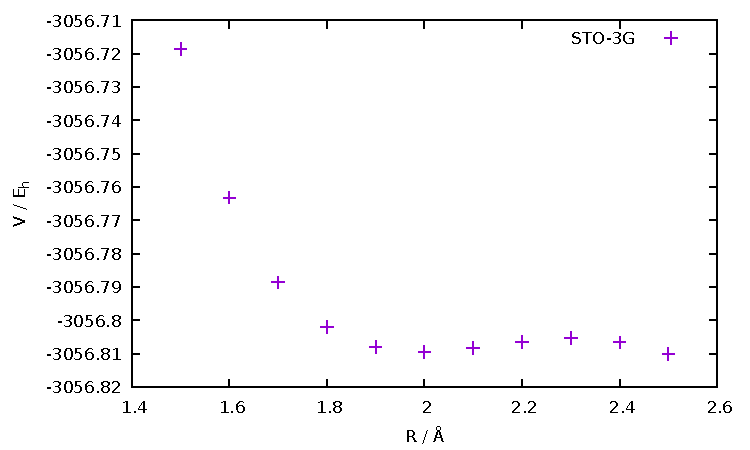
\includegraphics[width=\linewidth]{STO.pdf}
		\subcaption{Scanergebniss nach dem STO-3G Datensatz}
		\label{abb:STO}
	\end{subfigure}
	\hfill
	\begin{subfigure}{0.49\linewidth}
		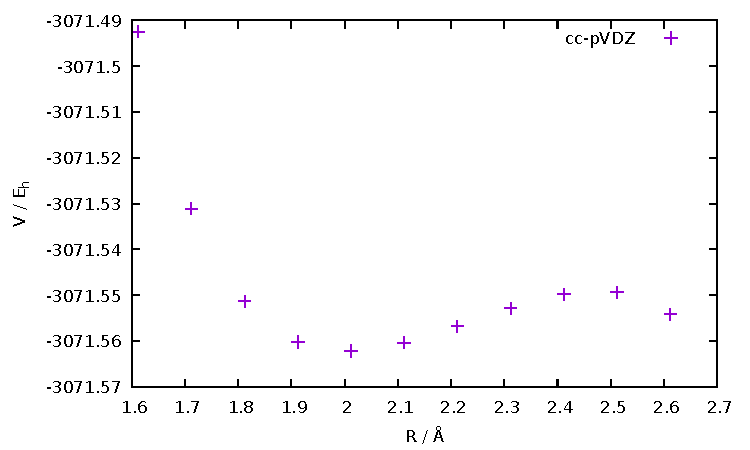
\includegraphics[width=\linewidth]{cc.pdf}
		\subcaption{Scanergebniss nach dem cc-pVDZ Datensatz}
 		\label{abb:cc}
	\end{subfigure}
	\caption{Totale Energie über Abstand der Reaktionspartner entlang der Reaktionskoordinate}
\end{figure}
Nach beendigung der Simulationen sind die in den Abbildungen \ref{abb:STO} und \ref{abb:cc}, sowie der Tabelle \ref{tab:AusgDaten} enthaltenen Daten erhalten worden.
Wie hier Zusehen wurden als erstes Nicht-SI-Einheiten in SI-Einheiten umgerechnet. 
Außerdem ist die elektronische Energie mit der Avogadrozahl multipliziert worden, um später eine molare Reaktionsenthalpie zu erhalten.
Dies vereinfacht im Weitern die Vergleichbarkeit.
Nach Gleichung \ref{eq:rktEnth} ist die Summe aus elektrischer Energie und die Nullpunktsschwingungsenergie die Reaktionsenthalpie.
\begin{equation}
H=EE+ZPVE
\label{eq:rktEnth}
\end{equation}

\begin{table}{b}
\centering
\begin{tabular}{rl|cccc}
Basissatz&         				& STO-3G              & STO-3G              & Cc-pVDZ             & Cc-pVDZ\\
Zustand	 &           				& Produkt             & Übergangszustand    & Produkt             & Übergangszustand\\
\hline
\hline
EE       &/\unit{\hartree} 			& -3038,27            & -3038,26            & -3071,58            & -3071,55\\
EE       &/\unit{\mega\joule\per\mole}   	& -7976,898           & -7976,866           & -8064,336           & -8064,268\\
ZPVE     &/\unit{\hartree}    			& 0,044               & 0,044               & 0,040               & 0,039\\
ZPVE     &/\unit{\joule\per\mole} 		& 116560,49	      & 115011,46           & 105685,78           & 102511,58\\
T        &/\unit{\kelvin}                	& 298,15              & 298,15              & 298,15              & 298,15\\
S        &/\unit{\cal\per\mole\per\kelvin}    	& 78,242              & 70,352              & 28,647              & 73,321\\
S        &/\unit{\joule\per\mole\per\kelvin}	& 327,36              & 294,35              & 119,86              & 306,78\\
\end{tabular}
\caption{Ausgangsdaten nach der Simulation der Reaktion}
\label{tab:AusgDaten}
\end{table}  

Weiter kann über die Gibbs-Gleichung (Gleichung \ref{eq:gibbs}) die gleichnamige Enthalpie (oder auch freie Reaktionsenthalpie genannt) errechnet werden.
\begin{equation}
G=H-T\Delta S
\label{eq:gibbs}
\end{equation}
Die Differenz der Gibbs-Energien zwischen Produkt und Übergangszustand gibt die Aktivierungsenergie.
Diese kann nun über die Arrheniusgleichung (Gleichung \ref{eq:arr}) in die dazugehörige Geschwindigkeitskonstante umgerechnet werden.
\begin{equation}
k=e^{\frac{-E_A}{R\cdot T}}
\label{eq:arr}
\end{equation}
Die Resultate dieser Rechnungen sind in Tabelle \ref{tab:res} dargestellt.
Der cc-pVDZ Basissatz ist generell größer und damit genauer.
Der STO-3G Datensatz zielt darauf ab, mit mathematischen Vereinfachungen einen Effizienten Überblick über die Energien zu bekommen \cite{sto}.
Während der cc-pVDZ Datensatz entwickelt wurde, mit dem Anspruch, möglichst komplett zu sein \cite{cc}.
Dies spiegelt sich zum Beispiel auch in der Rechenzeit wieder, welche hier deutlich länger gedauert haben. 
Zusehen ist dieser Unterschied unter anderem an den geringeren Energien, welche der cc-pVDZ Datensatz errechnet hat.
Nach dem Variationstheorem wird davon ausgegangen, das solche Simulationen stets einen zu großen Energiewert errechnen.
Somit sind niedrigere Ergebnisse immer näher an dem wahren Wert.
Weiter ist die errechnete Aktivierungsenergie sehr nah an den Literaturwerten.
Nach Tabelle \ref{tab:res} wurde über den cc-pVDZ Datensatz eine Aktivierungsenergie von \qty{9359,084}{\joule\per\mole} ermittelt werden.
Nach diesem\cite{geschk} Paper wird für diese Reaktion eine Aktivierungsenergie von \qty{-1,9}{\kilo\cal\per\mol} oder \qty{-7949,6}{\joule\per\mole}

\begin{table}
\centering
\begin{tabular}{rl|cccc}
\multicolumn{2}{c}{Basissatz}		   	& STO-3G        & STO-3G              & Cc-pVDZ              & Cc-pVDZ\\
\multicolumn{2}{c}{Zustand}			& Produkt       & Übergangszustand    & Produkt              & Übergangszustand\\
\hline
\hline
$H$             &/\unit{\mega\joule\per\mole} 	& -7976,78        & -7976,751   & -8064,231    & -8064,166\\
$G$             &/\unit{\mega\joule\per\mole}   & -7976,88        & -7976,839   & -8064,266    & -8064,257\\
$E_A$           &/\unit{\joule\per\mole} 	& \multicolumn{2}{c}{-40324,19}	& \multicolumn{2}{c}{-9359,084}\\
$k$             &/\unit{\per\second}       	& \multicolumn{2}{c}{\qty{8,62e-08}{}} & \multicolumn{2}{c}{0,0229}\\
\end{tabular}
\caption{Ergebnisse}
\label{tab:res}
\end{table}


\printbibliography
\end{document}
